%%%%%%%%%%%%%%%%%%%%%%%%%%%%%%%%%%%%%%%%%%%%%%%%%%%%%%%%%%%%%%%%%%%%%%%%%%%%%%%%%%
\begin{frame}[fragile]\frametitle{}
\begin{center}
{\Large Introduction to RASA Platform}

{\tiny (Ref: https://www.rasa.com/docs/getting-started/overview/ )}
\end{center}
\end{frame}



%%%%%%%%%%%%%%%%%%%%%%%%%%%%%%%%%%%%%%%%%%%%%%%%%%%%%%%%%%%
 \begin{frame}[fragile]\frametitle{Overview}
\begin{itemize}
\item The Rasa Stack is a pair of open source libraries (Rasa NLU and Rasa Core) that allow developers to expand chatbots and voice assistants beyond answering simple questions. 
\item Using state-of-the-art machine learning, your bots can hold contextual conversations with users. 
\item Rasa is production ready and used in large companies everywhere.
\end{itemize}


\end{frame}


%%%%%%%%%%%%%%%%%%%%%%%%%%%%%%%%%%%%%%%%%%%%%%%%%%%%%%%%%%%
 \begin{frame}[fragile]\frametitle{Who is it for?}
\begin{itemize}
\item The intended audience is mainly people developing bots, starting from scratch or looking to find a a drop-in replacement for wit, LUIS, or Dialogflow. 
\item The setup process is designed to be as simple as possible. 
\item Rasa NLU is written in Python, but you can use it from any language through a HTTP API. 
\item If your project is written in Python you can simply import the relevant classes. 
\item If you're currently using wit/LUIS/Dialogflow, you just:
\begin{itemize}
\item Download your app data from wit, LUIS, or Dialogflow and feed it into Rasa NLU
\item Run Rasa NLU on your machine and switch the URL of your wit/LUIS api calls to localhost:5000/parse
\end{itemize}
\end{itemize}
\end{frame}


% %%%%%%%%%%%%%%%%%%%%%%%%%%%%%%%%%%%%%%%%%%%%%%%%%%%%%%%%%%%
% \begin{frame}[fragile]\frametitle{Chatbot Workflow}

% \begin{itemize}
% \item Chatbot architecture is very similar to the architecture of a web application. 
% \item It works on the client-server model. 
% \item The differentiating factor is that it works with unstructured data.
% \end{itemize}

% % {\tiny (Ref: Chatbots 101 - Architecture \& Terminologies -  Bhavani Ravi)}
% \end{frame}


% %%%%%%%%%%%%%%%%%%%%%%%%%%%%%%%%%%%%%%%%%%%%%%%%%%%%%%%%%%%
% \begin{frame}[fragile]\frametitle{Chatbot Workflow}
% \begin{center}
% 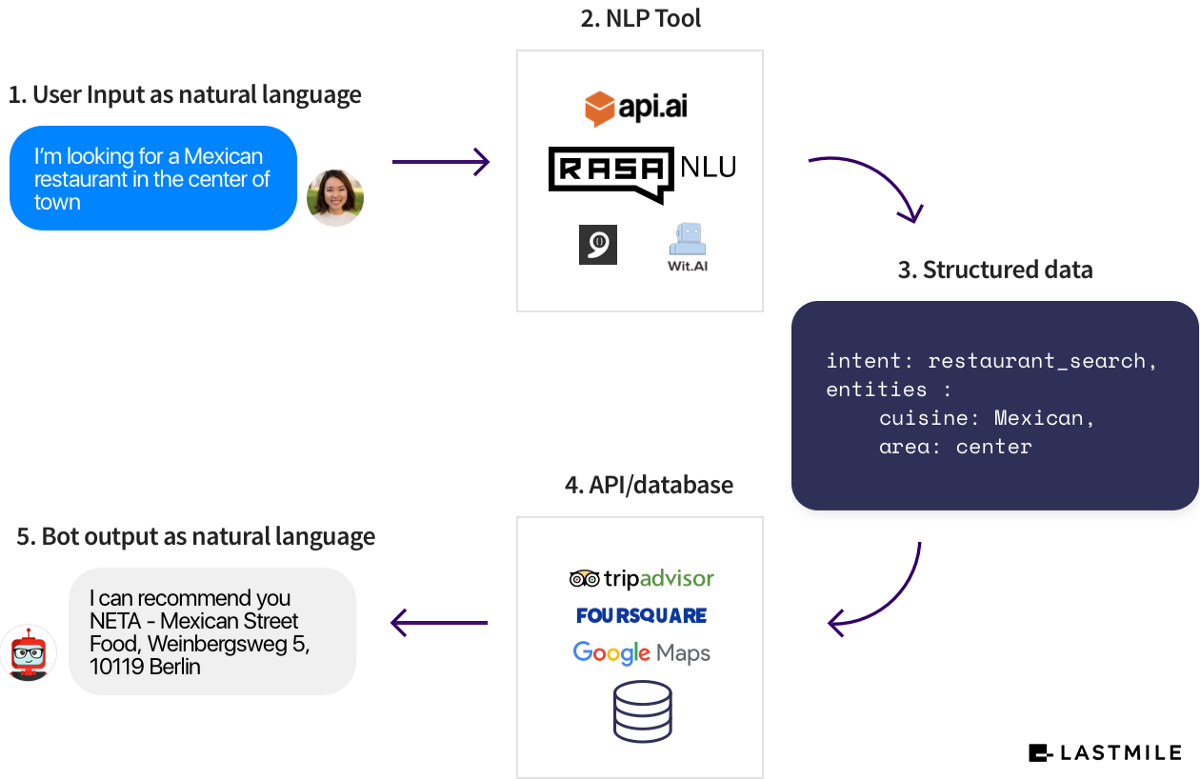
\includegraphics[width=0.9\linewidth]{rasa2}
% \end{center}

% % {\tiny (Ref: Chatbots 101 - Architecture \& Terminologies -  Bhavani Ravi)}
% \end{frame}


% %%%%%%%%%%%%%%%%%%%%%%%%%%%%%%%%%%%%%%%%%%%%%%%%%%%%%%%%%%%
% \begin{frame}[fragile]\frametitle{Differences with Web Apps?}

% \begin{itemize}
% \item In a web application, when you fill a form the data structure is constructed by the client in such a way that your server understands but, when it comes to chatbots, the client gets a raw text from a messaging interface(slack, FB messenger, etc.,). 
% \item In this case, you need a middle layer to parse the text and derive insights and call the respective backend API that performs the intended action.
% \end{itemize}

% % {\tiny (Ref: Chatbots 101 - Architecture \& Terminologies -  Bhavani Ravi)}
% \end{frame}

% %%%%%%%%%%%%%%%%%%%%%%%%%%%%%%%%%%%%%%%%%%%%%%%%%%%%%%%%%%%
 % \begin{frame}[fragile]\frametitle{Rasa Platform}
% \begin{center}
% 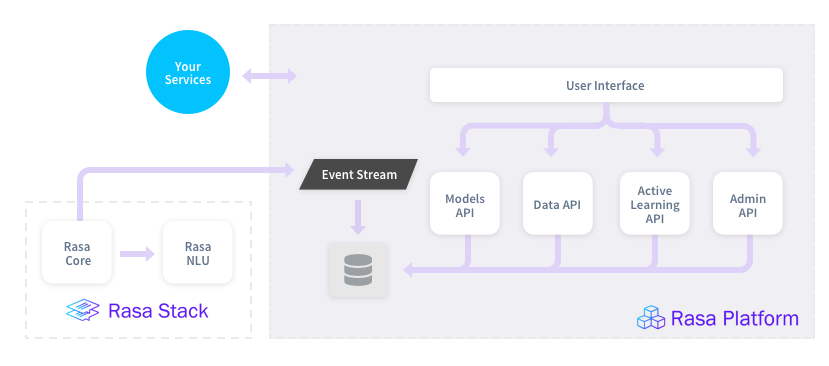
\includegraphics[width=\linewidth,keepaspectratio]{rasa-platform-diagram}
% \end{center}
% Rasa Platform extends the open source Rasa NLU and Rasa Core libraries with APIs, a graphical user interface, and our customer success program which includes enterprise-grade support.
% \end{frame}


%%%%%%%%%%%%%%%%%%%%%%%%%%%%%%%%%%%%%%%%%%%%%%%%%%%%%%%%%%%
 \begin{frame}[fragile]\frametitle{RASA Stack}
\begin{itemize}
\item Rasa NLU performs Natural Language Understanding, which means taking free-form text like
{\bf Please send the confirmation to amy@example.com}
and turning it into structured data. 
\item Rasa Core performs Dialog Management, which means keeping track of a conversation, and deciding how to proceed. 
\item Both Rasa Core and NLU use Machine Learning to learn from real example conversations.
\item Rasa NLU and Core are independent. You can use NLU without Core, and vice versa.
\end{itemize}
\end{frame}

%%%%%%%%%%%%%%%%%%%%%%%%%%%%%%%%%%%%%%%%%%%%%%%%%%%%%%%%%%%
 \begin{frame}[fragile]\frametitle{RASA Stack}
\begin{center}
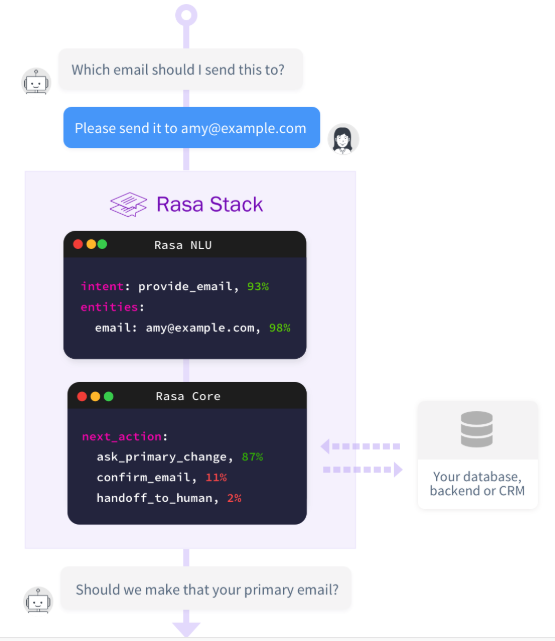
\includegraphics[width=0.5\linewidth,keepaspectratio]{chatbot3}
\end{center}

{\tiny (Ref: https://rasa.com/docs/get\_started\_step1/)}

\end{frame}


%%%%%%%%%%%%%%%%%%%%%%%%%%%%%%%%%%%%%%%%%%%%%%%%%%%%%%%%%%%
 \begin{frame}[fragile]\frametitle{RASA NLU Server}
\begin{itemize}
\item A RASA-NLU platform needs to be trained before we start using it. 
\item We need to supply it with a few sentences and mention which are the intents and entities in it.
\end{itemize}
\end{frame}


%%%%%%%%%%%%%%%%%%%%%%%%%%%%%%%%%%%%%%%%%%%%%%%%%%%%%%%%%%%
 \begin{frame}[fragile]\frametitle{Summary: The Rasa Stack}
Rasa NLU's job is to interpret messages, and Rasa Core's job is to decide what should happen next.

\begin{center}
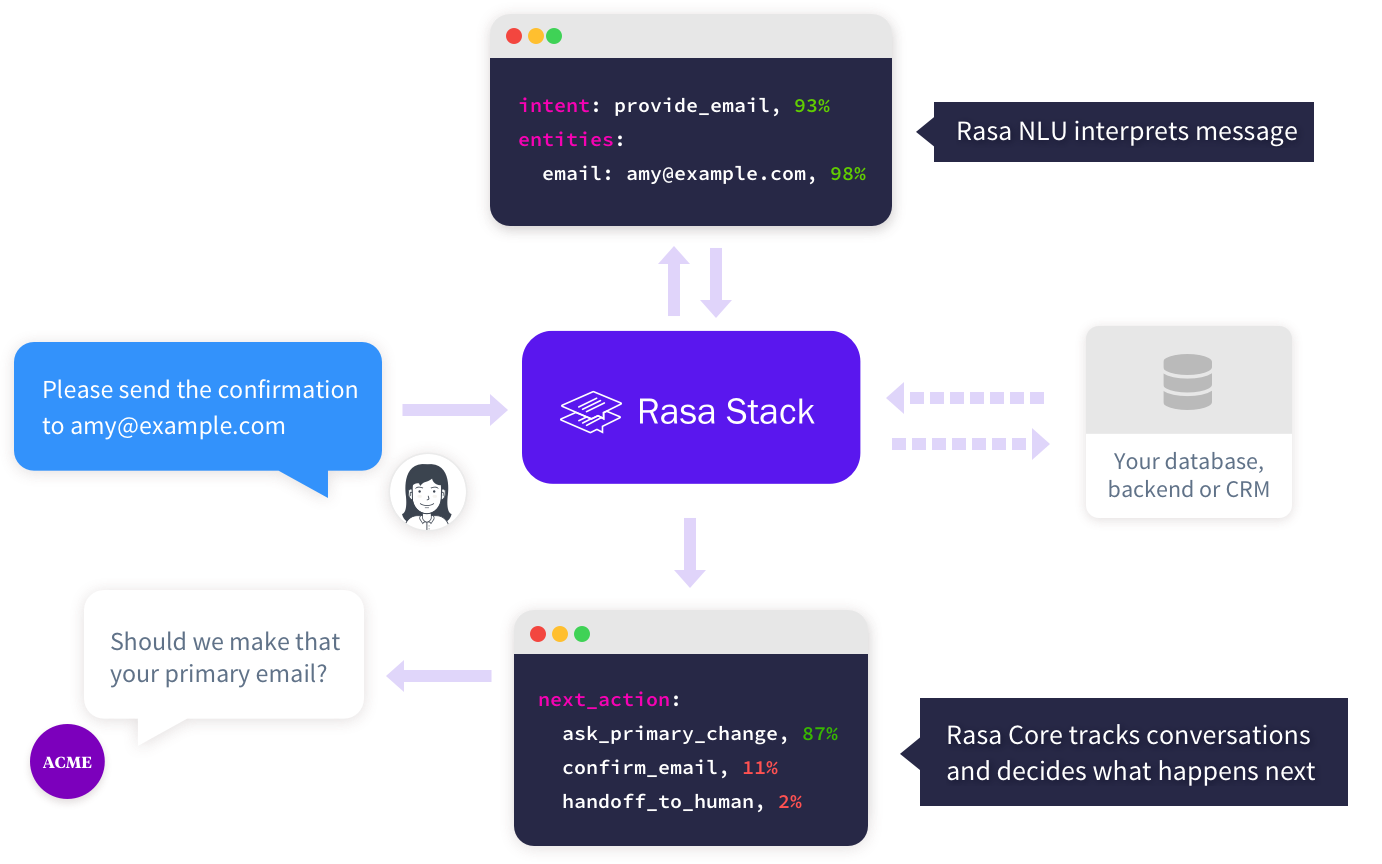
\includegraphics[width=0.8\linewidth,keepaspectratio]{rasa_stack_explained}
\end{center}

\end{frame}


